\documentclass{beamer}
\usepackage[utf8]{inputenc}
\usetheme{Berlin}
\usepackage{tikz}
\title{Binary Heap}
\author[1805068, 1805067]{Showvik Biswas\\Muhammad Ehsanul Kader}
\institute{Department of CSE, BUET}
\date{\today}

\begin{document}

\frame{\titlepage}

\section{A Problem in Context}

\frame{\tableofcontents[currentsection]}

\begin{frame}{The 14th Week of BUET}
\begin{itemize}
    \item One of the most gruesome experiences an undergraduate student at BUET can ever have.
    \pause
    \item So much to be done, with such limited time!
\end{itemize}
\end{frame}

\begin{frame}{To-Do List}
    \begin{figure}
        \centering
        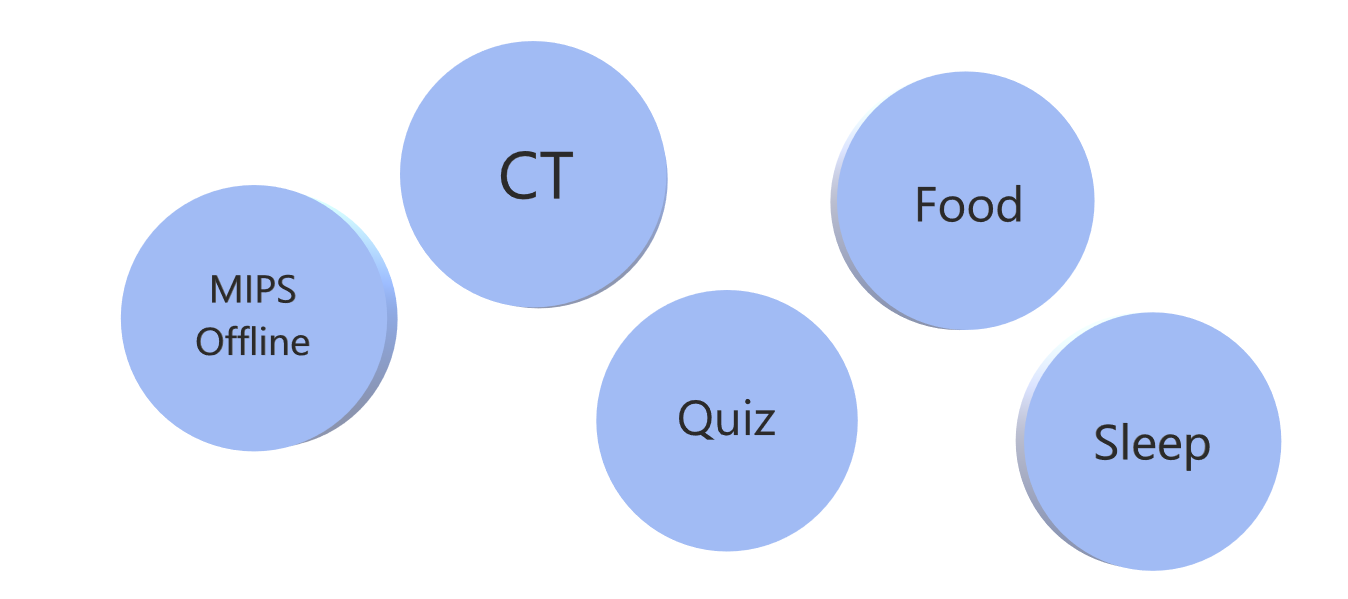
\includegraphics[scale=0.25]{1.png}
        \caption{A few things to be done}
        \label{fig:my_label}
    \end{figure}
\end{frame}
\section{Solving the Problem}
\frame{\tableofcontents[currentsection]}
\begin{frame}{Possible Solution}
\begin{itemize}
    \item Sort by priority?
    \pause
    \item Most prioritized task available.
    \pause
    \item Results in something called a \textbf{priority queue}.
\end{itemize}
\pause
\begin{definition}
A priority queue is an abstract data-type in which each element has a priority associated with it.
\end{definition}
\end{frame}

\begin{frame}{The Priority Queue}
    \begin{figure}
        \centering
        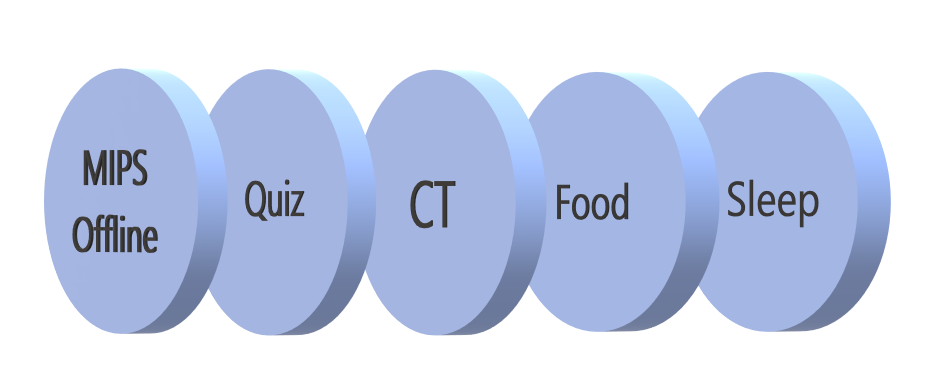
\includegraphics[scale=0.3]{2.png}
        \caption{Sorting the tasks according to their respective priorities...}
        \label{fig:my_label}
    \end{figure}
\end{frame}

\begin{frame}{The Priority Queue}
    \begin{figure}
        \centering
        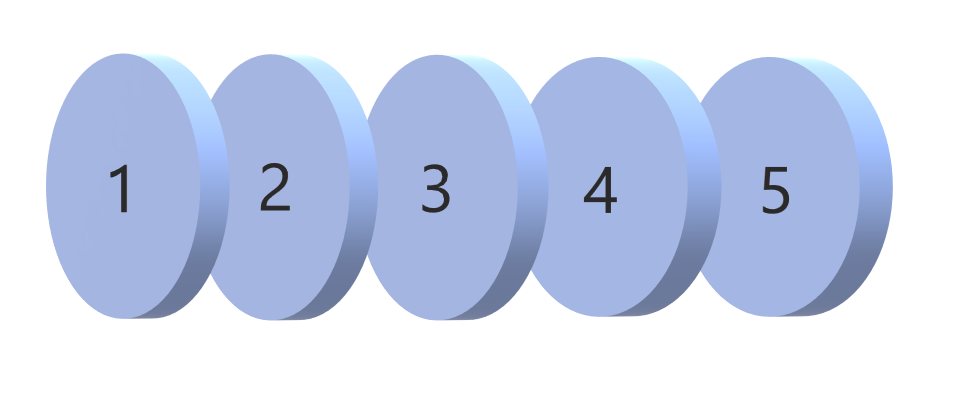
\includegraphics[scale=0.3]{3.png}
        \caption{...and assigning them priority numbers}
        \label{fig:my_label}
    \end{figure}
\end{frame}

\begin{frame}{Implementing the Priority Queue}
\begin{itemize}
    \item Most plausible option seems an array
\end{itemize}
\pause
\begin{figure}
    \centering
    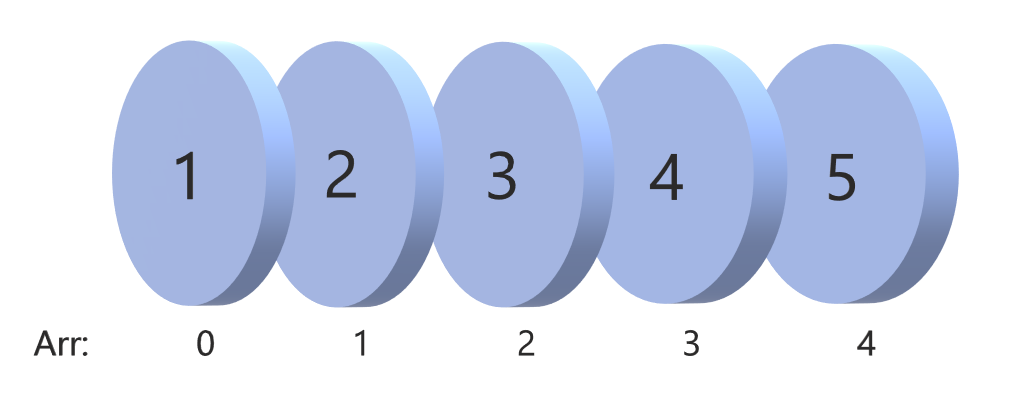
\includegraphics[scale=0.25]{5.png}
    \caption{Array Implementation of PQ}
    \label{fig:my_label}
\end{figure}
\end{frame}

\begin{frame}{The Catch}
    \begin{itemize}
        \item What if a more important task comes along?
    \end{itemize}
    \pause
    \begin{figure}
        \centering
        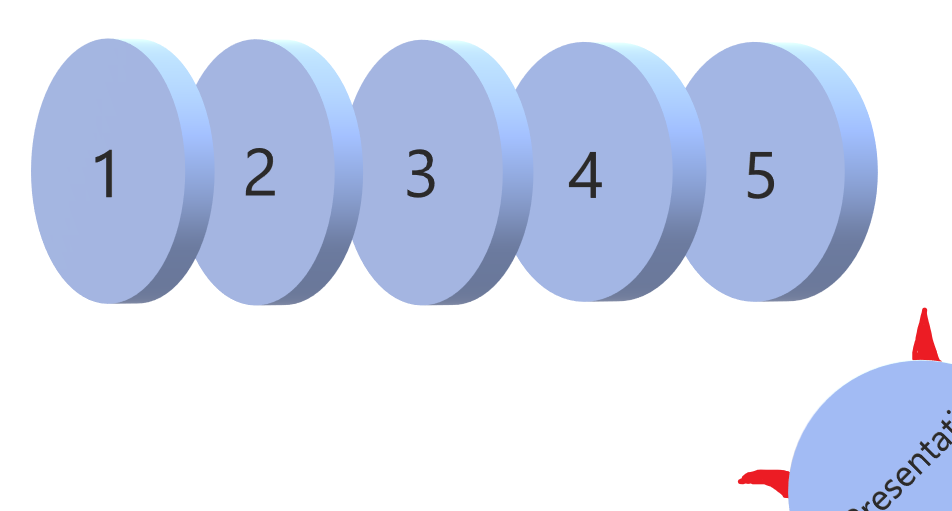
\includegraphics[scale=0.3]{4.png}
        \caption{The \LaTeX presentation is obviously the most prioritized}
        \label{fig:my_label}
    \end{figure}
\end{frame}

\begin{frame}{An Alternative}
    \begin{itemize}
        \item The array will have to be resorted, and this will be a trouble with limited storage and time.
        \item A better alternative: \textbf{binary heaps}.
    \end{itemize}
\end{frame}

\begin{frame}{Binary Heap: Definition}
    \item A binary heap is a binary tree with \textbf{two invariants}.
    \begin{enumerate}
        \item Every node is smaller (for min-heaps), or bigger (for max-heaps) than its descendant nodes.
        \item The left sub-tree of a node must have an equal number of nodes, or have one more node than the right sub-tree.
    \end{enumerate}
\end{frame}

\begin{frame}{A binary heap}
    \begin{figure}
        \centering
        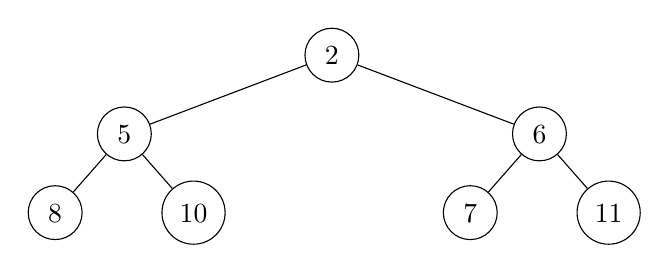
\begin{tikzpicture}[baseline,
  level distance=10mm,
  text depth=.1em,
  text height=.8em,
  level 1/.style={sibling distance=15em},
  level 2/.style={sibling distance=5em},
  level 3/.style={sibling distance=5em},
  level 4/.style={sibling distance=10em}]
\node[circle,draw](z){2}
  child{node[circle,draw]{5} child{node[circle,draw] {8}} child{node[circle,draw] {10}}}
  child{
    node[circle,draw]{6} child{node[circle,draw] {7}} child{node[circle,draw] {11}} };
\end{tikzpicture}
        \caption{Binary Heap}
        \label{fig:my_label}
    \end{figure}
\end{frame}
\section{Binary Heap Operations}
\frame{\tableofcontents[currentsection]}
\begin{frame}{Binary Heap: Operations}
    \begin{itemize}
        \item \textcolor<2>{red}{Insertion}
        \item \textcolor<2>{red}{Extract Min}
        \item Find Min
        \item Deletion
        \item Decrease or increase key
    \end{itemize}
\end{frame}

\begin{frame}{Insertion}
    \begin{block}{Insertion Steps}
    \begin{itemize}
        \item Place the new node in the next available spot
        \item Push the new node upwards until heap property is satisfied.
    \end{itemize}
\end{block}
\end{frame}



\begin{frame}{Insertion}
    \begin{figure}
        \centering
        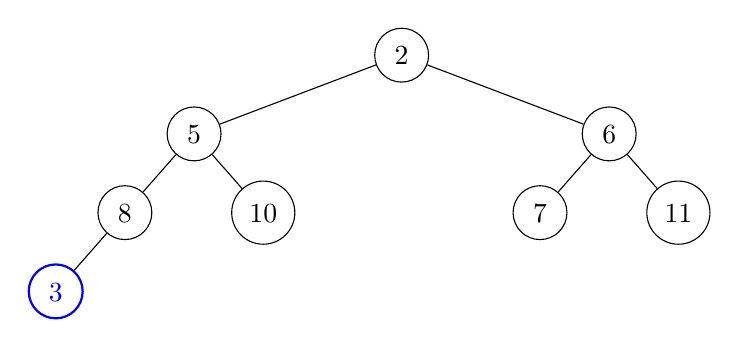
\begin{tikzpicture}[baseline,
  level distance=10mm,
  text depth=.1em,
  text height=.8em,
  level 1/.style={sibling distance=15em},
  level 2/.style={sibling distance=5em},
  level 3/.style={sibling distance=5em},
  level 4/.style={sibling distance=10em}]
\node[circle,draw](z){2}
  child{node[circle,draw]{5} child{node[circle,draw] {8}  child{node[circle,draw,blue,thick] {3}} child[missing]} child{node[circle,draw] {10}}}
  child{
    node[circle,draw]{6} child{node[circle,draw] {7} } child{node[circle,draw] {11}} };
\end{tikzpicture}
        \caption{Inserting 3}
        \label{fig:my_label}
    \end{figure}
\end{frame}

\begin{frame}{Insertion}
    \begin{figure}
        \centering
        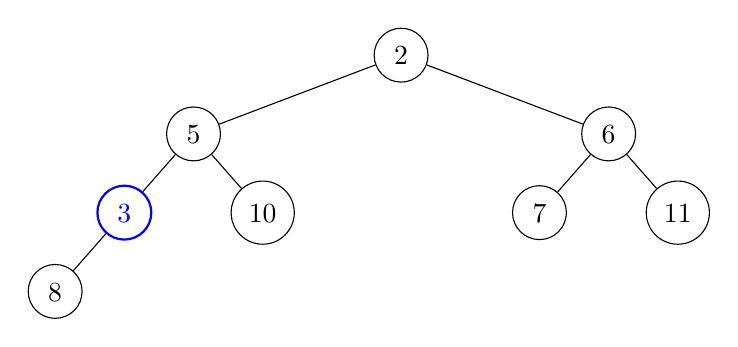
\begin{tikzpicture}[baseline,
  level distance=10mm,
  text depth=.1em,
  text height=.8em,
  level 1/.style={sibling distance=15em},
  level 2/.style={sibling distance=5em},
  level 3/.style={sibling distance=5em},
  level 4/.style={sibling distance=10em}]
\node[circle,draw](z){2}
  child{node[circle,draw]{5} child{node[circle,draw,blue,thick] {3}  child{node[circle,draw] {8}} child[missing]} child{node[circle,draw] {10}}}
  child{
    node[circle,draw]{6} child{node[circle,draw] {7} } child{node[circle,draw] {11}} };
\end{tikzpicture}
        \caption{Restoring heap property}
        \label{fig:my_label}
    \end{figure}
\end{frame}

\begin{frame}{Insertion}
    \begin{figure}
        \centering
        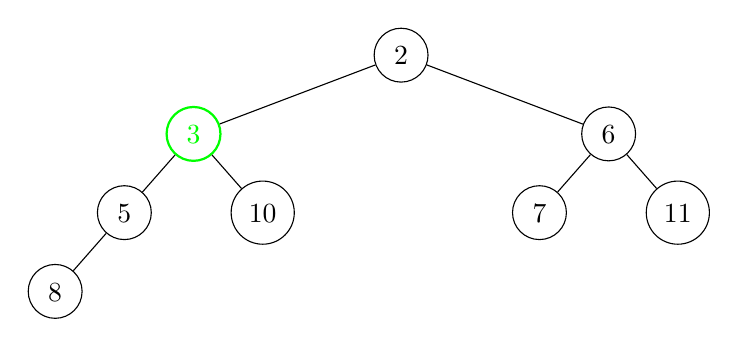
\begin{tikzpicture}[baseline,
  level distance=10mm,
  text depth=.1em,
  text height=.8em,
  level 1/.style={sibling distance=15em},
  level 2/.style={sibling distance=5em},
  level 3/.style={sibling distance=5em},
  level 4/.style={sibling distance=10em}]
\node[circle,draw](z){2}
  child{node[circle,draw,green,thick]{3} child{node[circle,draw] {5}  child{node[circle,draw] {8}} child[missing]} child{node[circle,draw] {10}}}
  child{
    node[circle,draw]{6} child{node[circle,draw] {7} } child{node[circle,draw] {11}} };
\end{tikzpicture}
        \caption{Restoring heap property}
        \label{fig:my_label}
    \end{figure}
\end{frame}

\begin{frame}{Extract Min}
    \begin{block}{Extract Min}
    \begin{itemize}
        \item Place the last node on the root.
        \item Push the out of place node downwards until heap property is satisfied (Heapify)
    \end{itemize}
\end{block}
\end{frame}


\begin{frame}{Extract Min}
    \begin{figure}
        \centering
        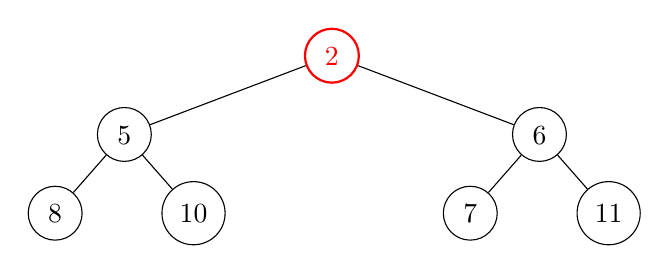
\begin{tikzpicture}[baseline,
  level distance=10mm,
  text depth=.1em,
  text height=.8em,
  level 1/.style={sibling distance=15em},
  level 2/.style={sibling distance=5em},
  level 3/.style={sibling distance=5em},
  level 4/.style={sibling distance=10em}]
\node[circle,draw,red,thick](z){2}
  child{node[circle,draw]{5} child{node[circle,draw] {8}} child{node[circle,draw] {10}}}
  child{
    node[circle,draw]{6} child{node[circle,draw] {7}} child{node[circle,draw] {11}} };
\end{tikzpicture}
        \caption{Place last element on root}
        \label{fig:extract_min1}
    \end{figure}
\end{frame}


\begin{frame}{Extract Min}
    \begin{figure}
        \centering
        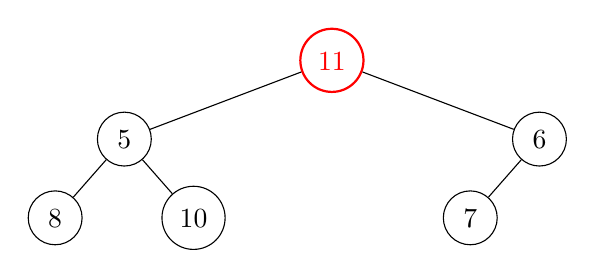
\begin{tikzpicture}[baseline,
  level distance=10mm,
  text depth=.1em,
  text height=.8em,
  level 1/.style={sibling distance=15em},
  level 2/.style={sibling distance=5em},
  level 3/.style={sibling distance=5em},
  level 4/.style={sibling distance=10em}]
\node[circle,draw,red,thick](z){11}
  child{node[circle,draw]{5} child{node[circle,draw] {8}} child{node[circle,draw] {10}}}
  child{
    node[circle,draw]{6} child{node[circle,draw] {7}} child[missing] };
\end{tikzpicture}
        \caption{Heapify after extracting}
        \label{fig:extract_min3}
    \end{figure}
\end{frame}

\begin{frame}{Extract Min}
    \begin{figure}
        \centering
        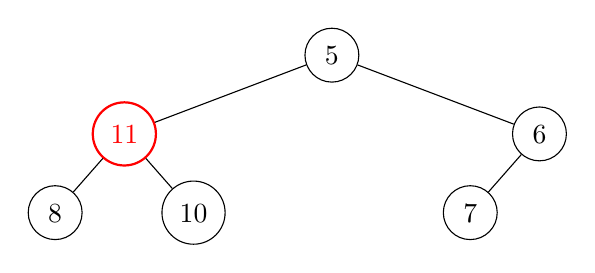
\begin{tikzpicture}[baseline,
  level distance=10mm,
  text depth=.1em,
  text height=.8em,
  level 1/.style={sibling distance=15em},
  level 2/.style={sibling distance=5em},
  level 3/.style={sibling distance=5em},
  level 4/.style={sibling distance=10em}]
\node[circle,draw](z){5}
  child{node[circle,draw,red,thick]{11} child{node[circle,draw] {8}} child{node[circle,draw] {10}}}
  child{
    node[circle,draw]{6} child{node[circle,draw] {7}} child[missing] };
\end{tikzpicture}
        \caption{Heapify after extracting}
        \label{fig:extract_min4}
    \end{figure}
\end{frame}

\begin{frame}{Extract Min}
    \begin{figure}
        \centering
        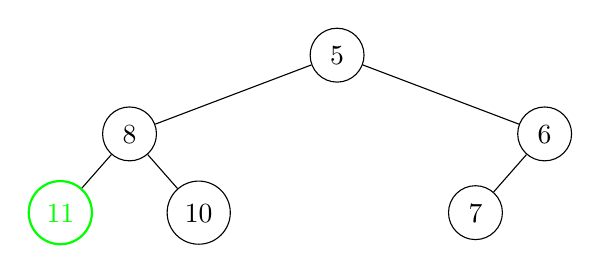
\begin{tikzpicture}[baseline,
  level distance=10mm,
  text depth=.1em,
  text height=.8em,
  level 1/.style={sibling distance=15em},
  level 2/.style={sibling distance=5em},
  level 3/.style={sibling distance=5em},
  level 4/.style={sibling distance=10em}]
\node[circle,draw](z){5}
  child{node[circle,draw]{8} child{node[circle,draw,green,thick] {11}} child{node[circle,draw] {10}}}
  child{
    node[circle,draw]{6} child{node[circle,draw] {7}} child[missing] };
\end{tikzpicture}
        \caption{Heapify after extracting}
        \label{fig:extract_min5}
    \end{figure}
\end{frame}

\begin{frame}{Time Complexity}
\begin{table}[]
    \centering
    \begin{tabular}{|c|c|}
        \hline
    	Operation & Time Complexity \\
    	\hline
    	 Insert Value & $O(\log{}n)$ \\
    	\hline
    	Extract Min & $O(\log{}n)$ \\
    	\hline
    \end{tabular}
    
\end{table}

\end{frame}

\begin{frame}{}
    \Huge
    \centering
    Thank You!
\end{frame}

\end{document}
